% 导言区
\documentclass{article}
\usepackage{ctex}  % 添加中文包
\usepackage{multirow} % 表格单元占据多个行或者列
\usepackage{listings} % 插入代码
\usepackage{xcolor}
\lstset{    % 设置代码样式
	numbers=left, 
	numberstyle= \tiny, 
	keywordstyle= \color{ blue!70},
	commentstyle= \color{red!50!green!50!blue!50}, 
	frame=shadowbox, % 阴影效果
	rulesepcolor= \color{ red!20!green!20!blue!20} ,
	escapeinside=``, % 英文分号中可写入中文
	xleftmargin=2em,xrightmargin=2em, aboveskip=1em,
	framexleftmargin=2em
} 
\usepackage{amssymb} % 和数学公式有关的包
\usepackage{graphicx} % 插入图片
\usepackage{subfigure} % 子图
\title{ICS homework6} 
\author{张运吉 211300063} 
\date{20/12/2022}

% 正文区 
\begin{document} 
\maketitle % 必须有这个才能显示标题等信息
\begin{center}
    \textbf{第七章作业}
\end{center}
\section*{P3}
都是并发的。
\section*{P4}
\subsection*{(1)}
不会。因为第一条指令的虚拟地址是0x80482c0,低12位不是全0,所以并不是某一页的开始,
所以,执行第一条指令前面的某条指令是,上述7条指令同时被装入内存,所以不会有缺页异常。
\subsection*{(2)}
第1条指令:数据访问会发生缺页,但是是可恢复的故障。因为b[1000]的地址是0x80497d0,访问b[1000]时是对所在页面的第一次
访问,此时该页面并未被调入内存中。CPU检测到缺页异常,暂停进程P,交给操作系统处理,操作系统在检查没有地址
越界或者越权访问后(这里显然没有),把该缺失的页从外存调入内存,处理结束后,回到movl指令重新执行,此时,
再次访问b[1000]就没有问题了。

第2条指令:同一,访问0x804a324时是对所在页的第一次访问,会发生和(1)一样的故障,
处理过程和结果也如同(1).

第6条指令:不会发生异常,因为在第2条指令时已经访问过地址0x804a324了,所在页已经在内存中,
所以不会发生缺页故障。

第7条指令:会发生故障,因为b[10000]并不存在,且计算出的地址0x804de20已经偏离数组首地址20002个单元,
很可能超出了读写数据区的范围。当CPU处理该指令时,发生缺页异常,交给操作系统处理,如果超出了读写数据区
的范围,操作系统会检测到地址越界或者越权访问,会发送“段错误”的信号给用户进程,并终止用户进程。这属于不可恢复的故障。

\begin{figure}[htbp]
	\centering
	\subfigure[Fig1]{
	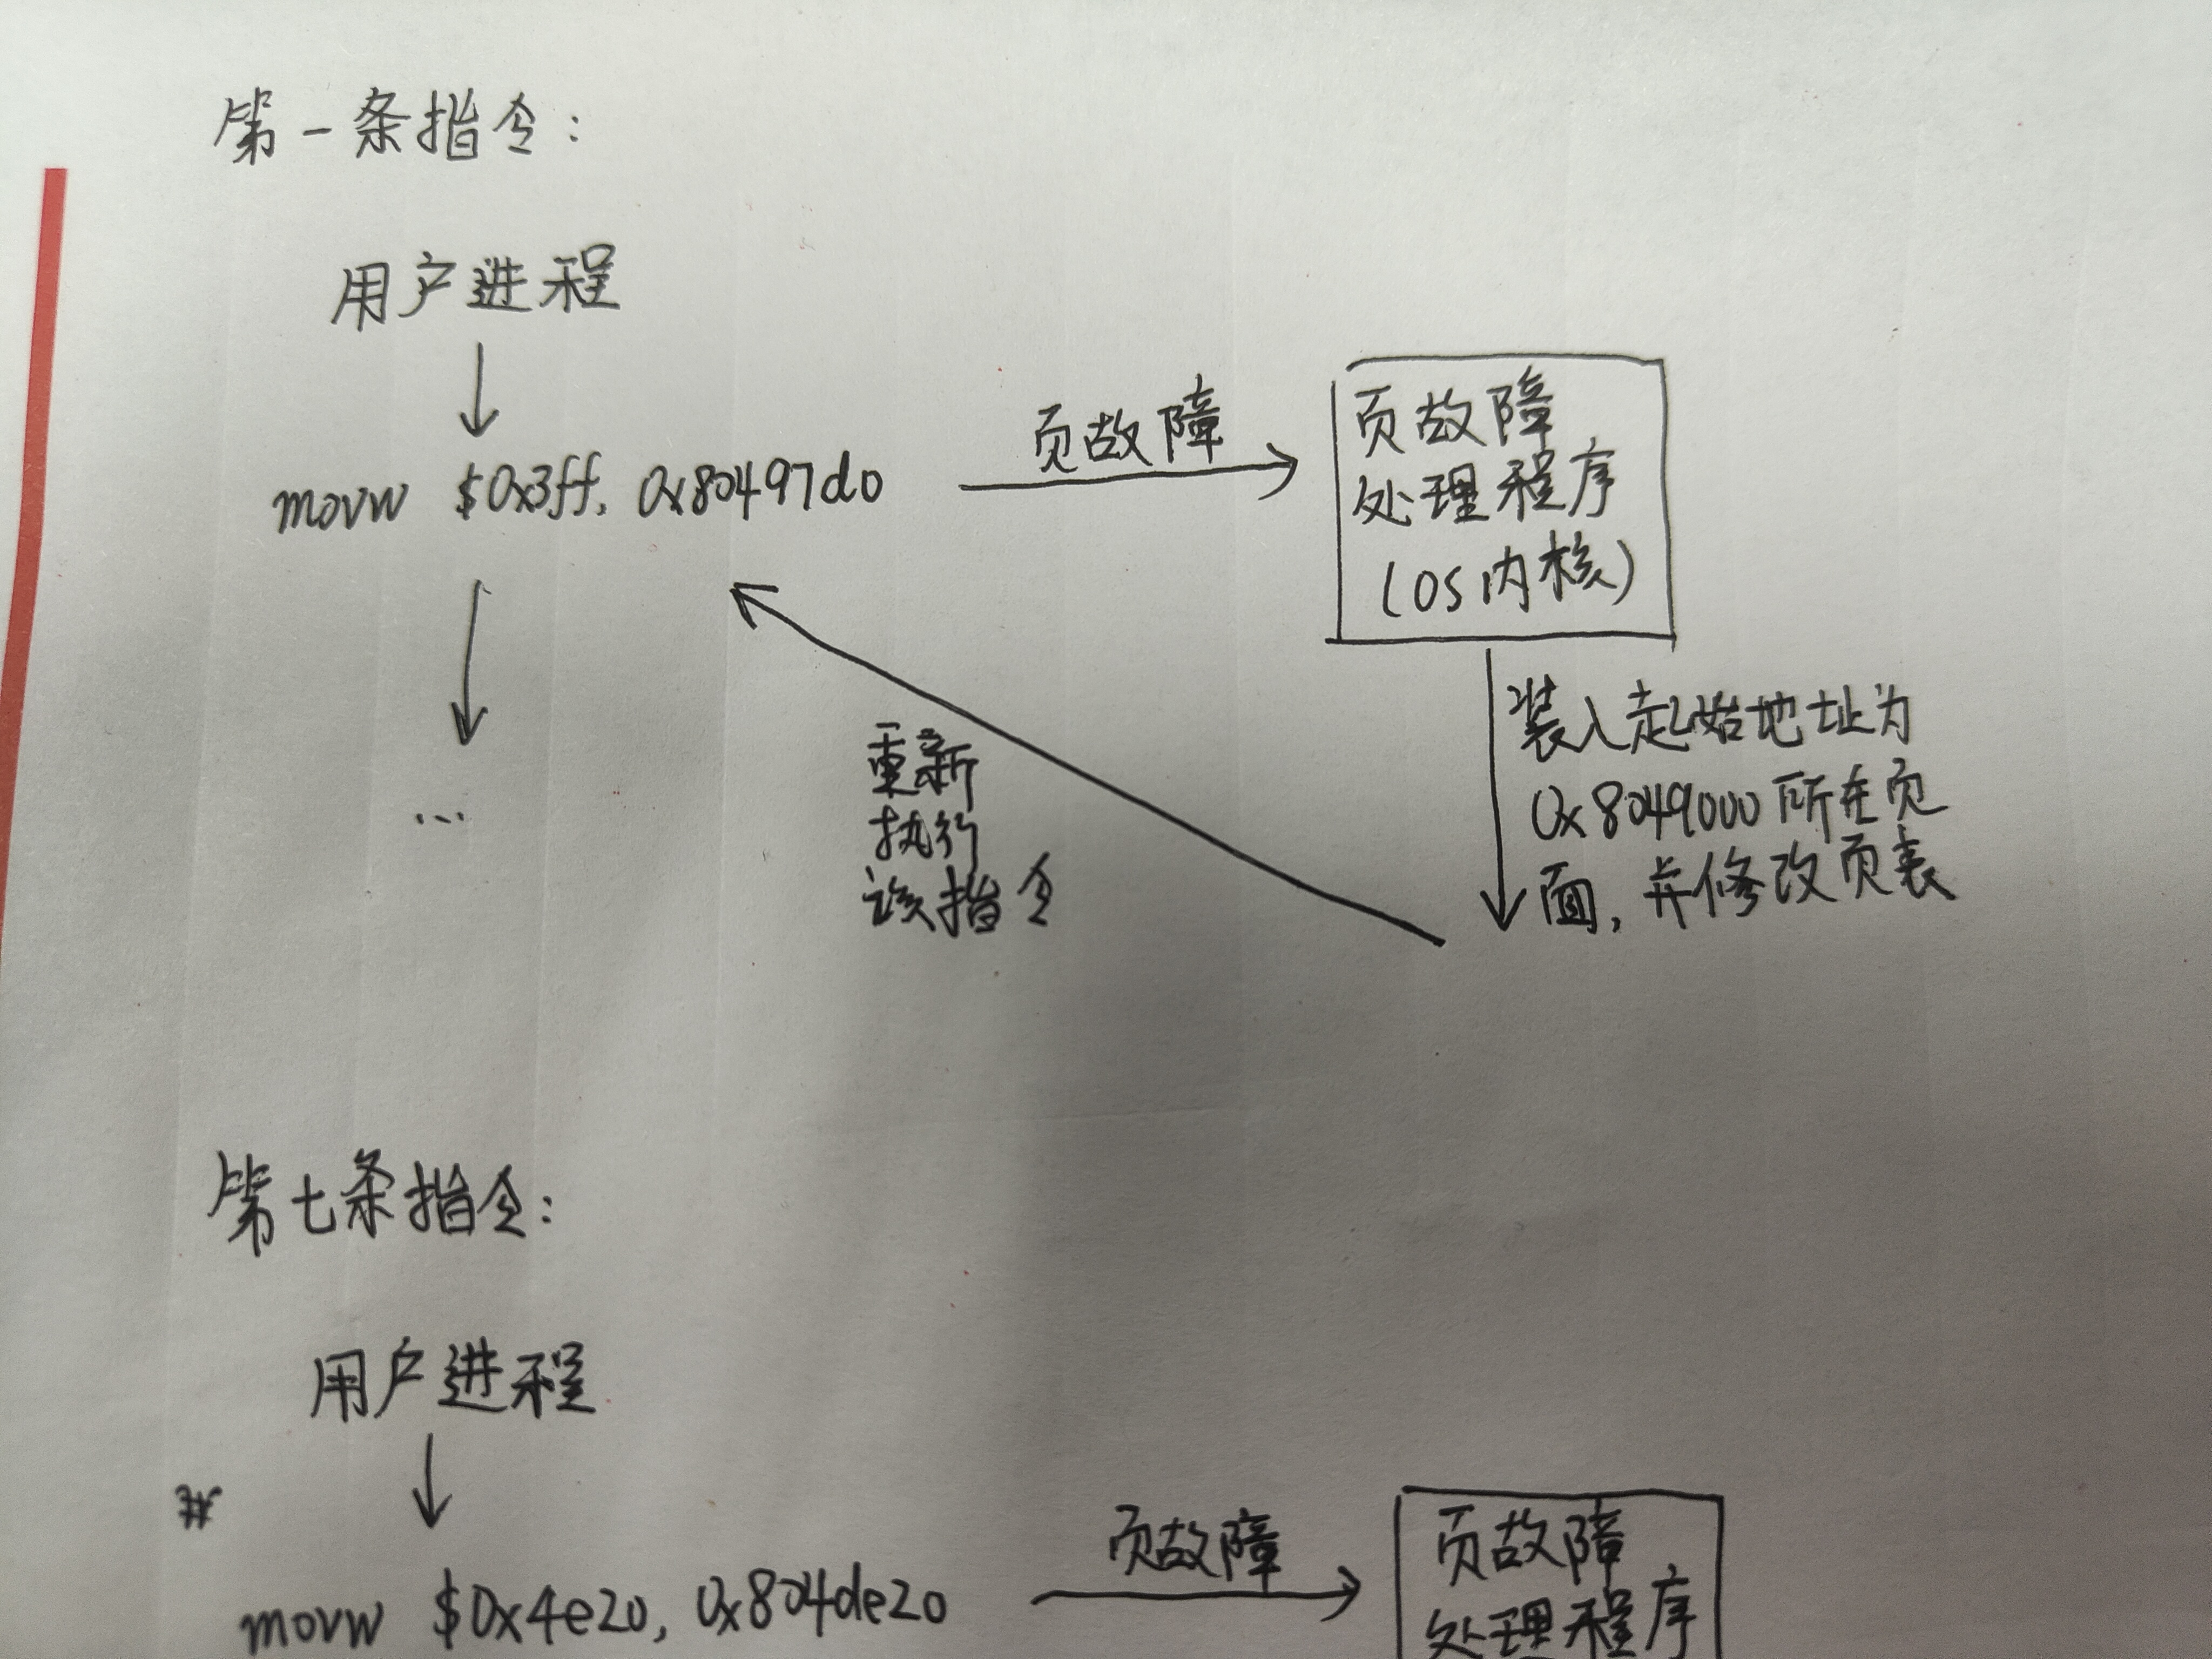
\includegraphics[width=4cm,height=4cm]{1.jpg} \label{1}
	}
	\quad
	\subfigure[Fig2]{
	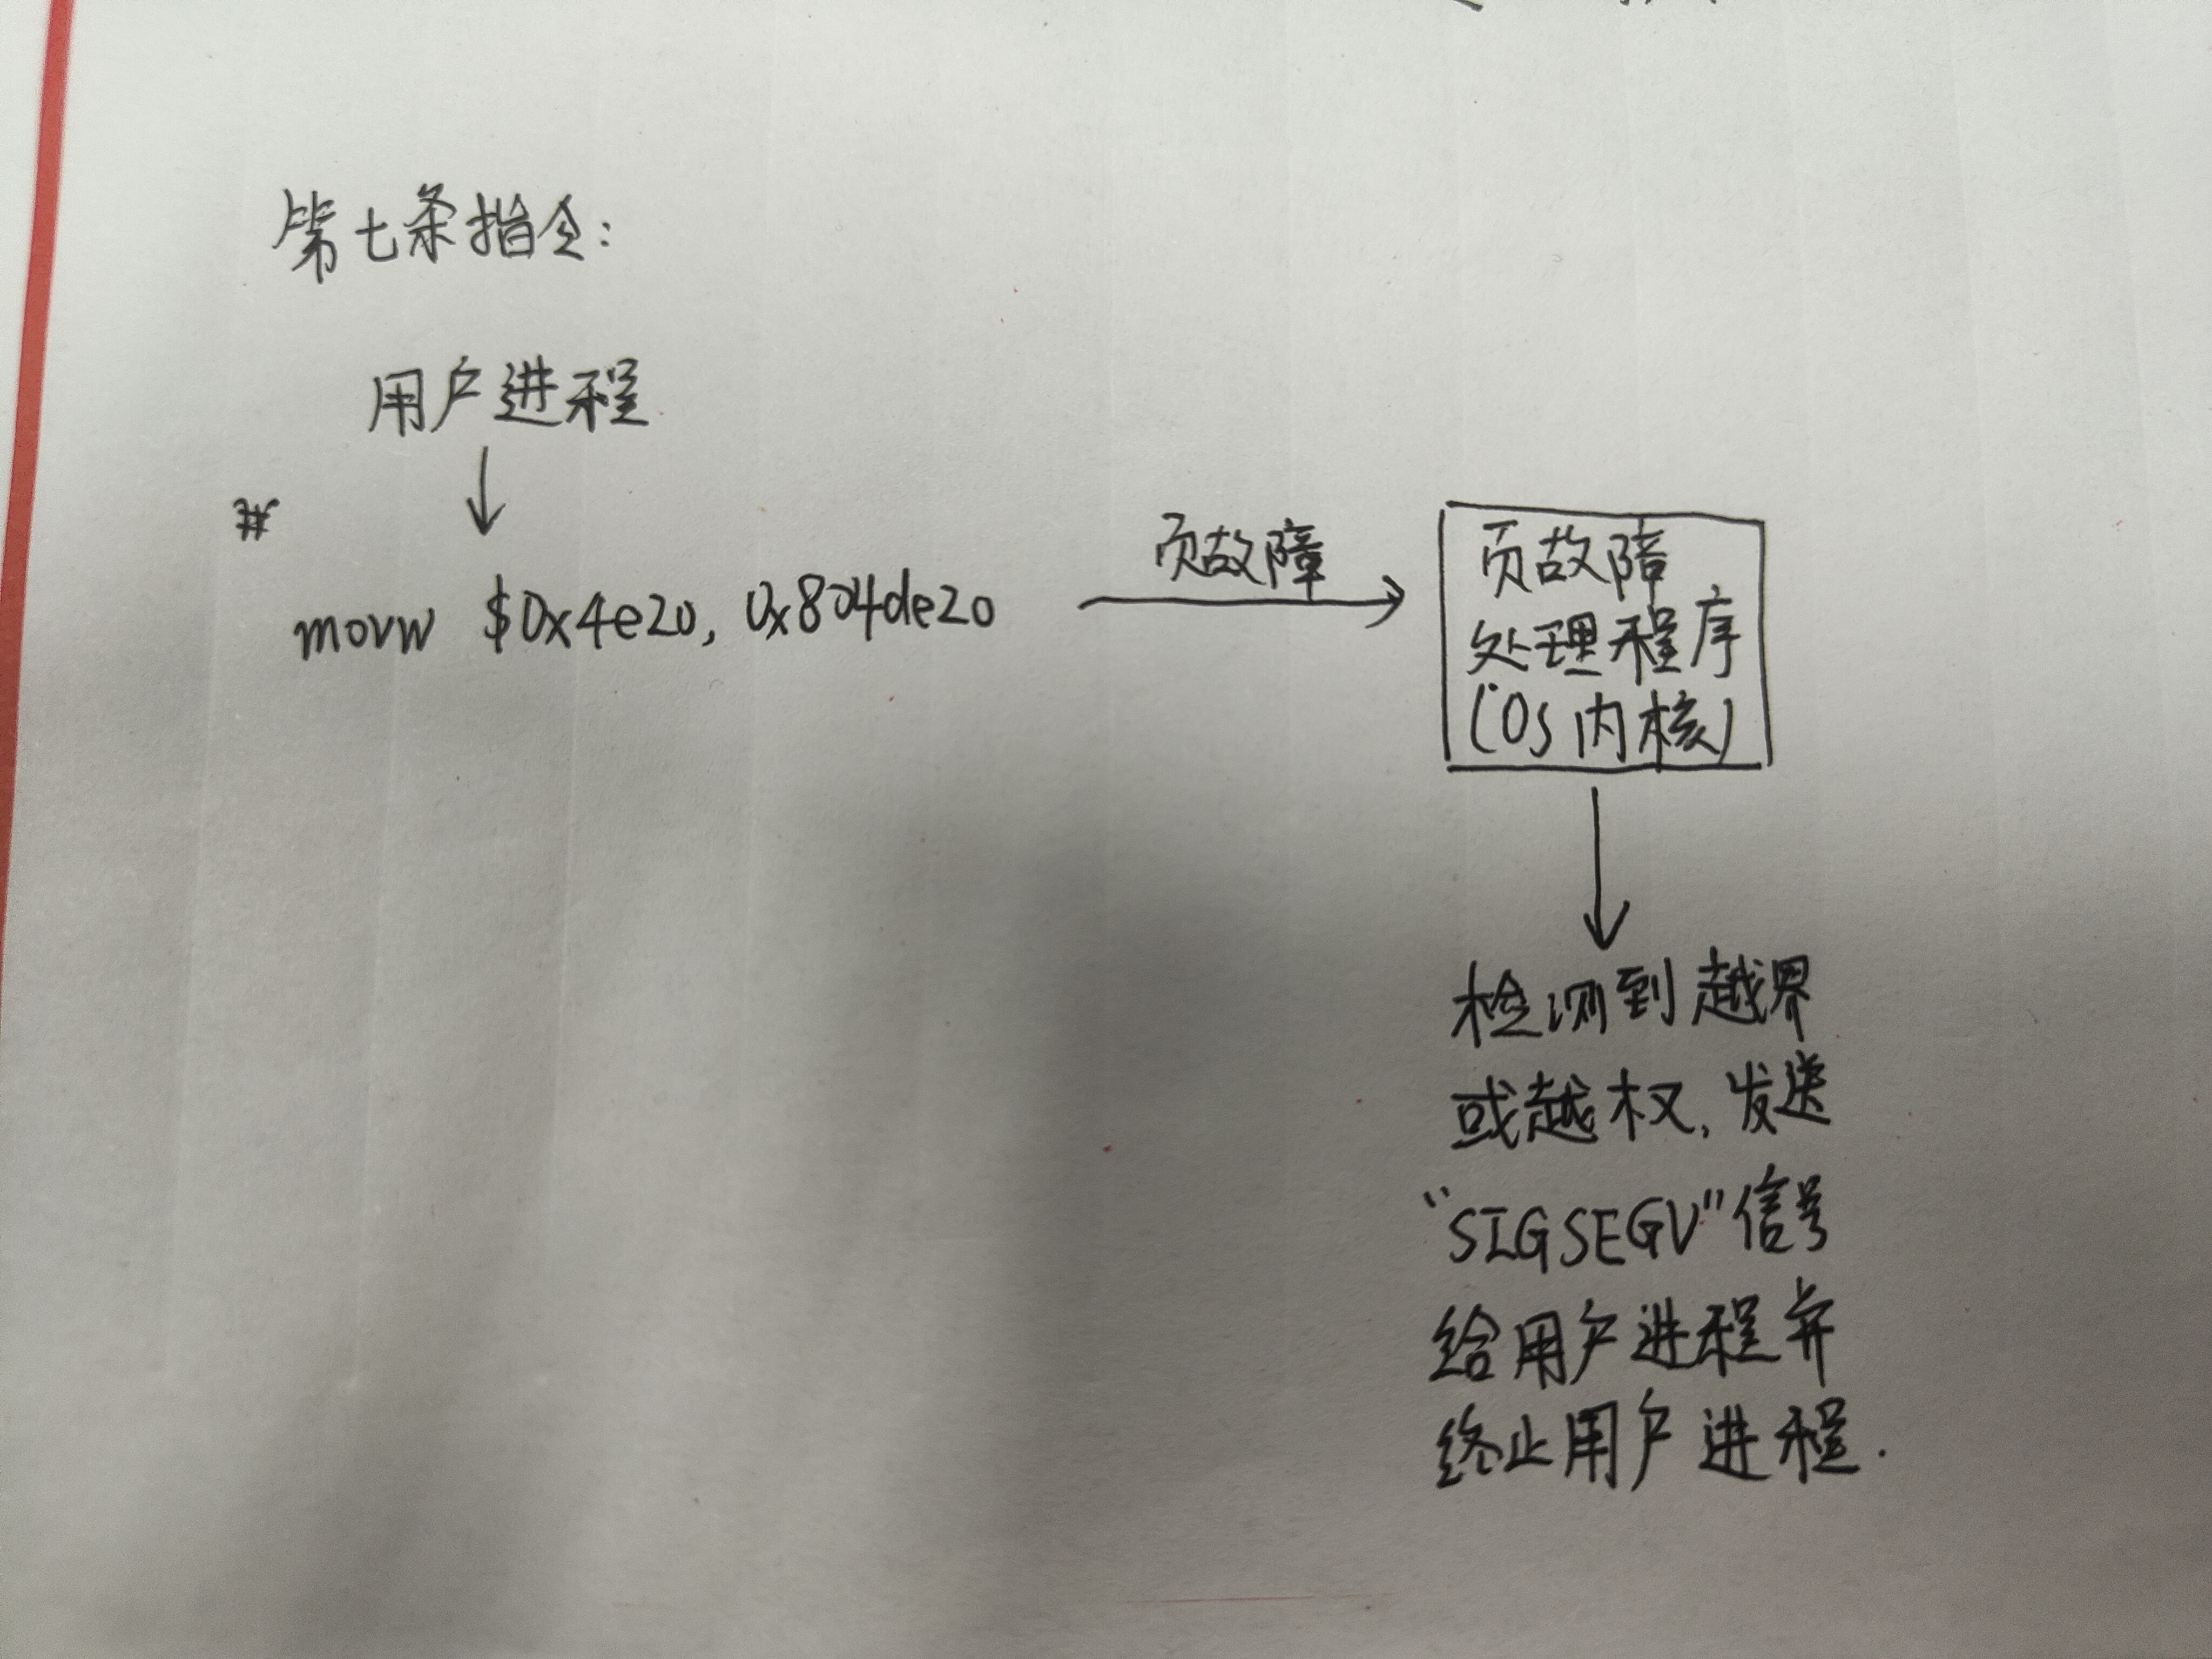
\includegraphics[width=4cm,height=4cm]{7.jpg} \label{2} 
	}
\end{figure}
\subsection*{(3)}
这里忘记给k赋初值,k是未初始化的全局变量,存在.bss节中,通常会将.bss节中的变量自动
初始化位0,所以这里会发生“整除0”故障,该故障不可恢复。
\newpage
\begin{center}
    \textbf{第八章作业}
\end{center}
\section*{P3}
\subsection*{(1)}
该程序的功能是在标准输出设备上输出"Hello, World."
\subsection*{(2)}
第16,20行指令。
\subsection*{(3)}
第16行指令调用4号系统调用write,第20行指令调用1号系统调用exit。
\section*{P4}
\subsection*{(1)}
\begin{figure}[htbp]
	\centering
	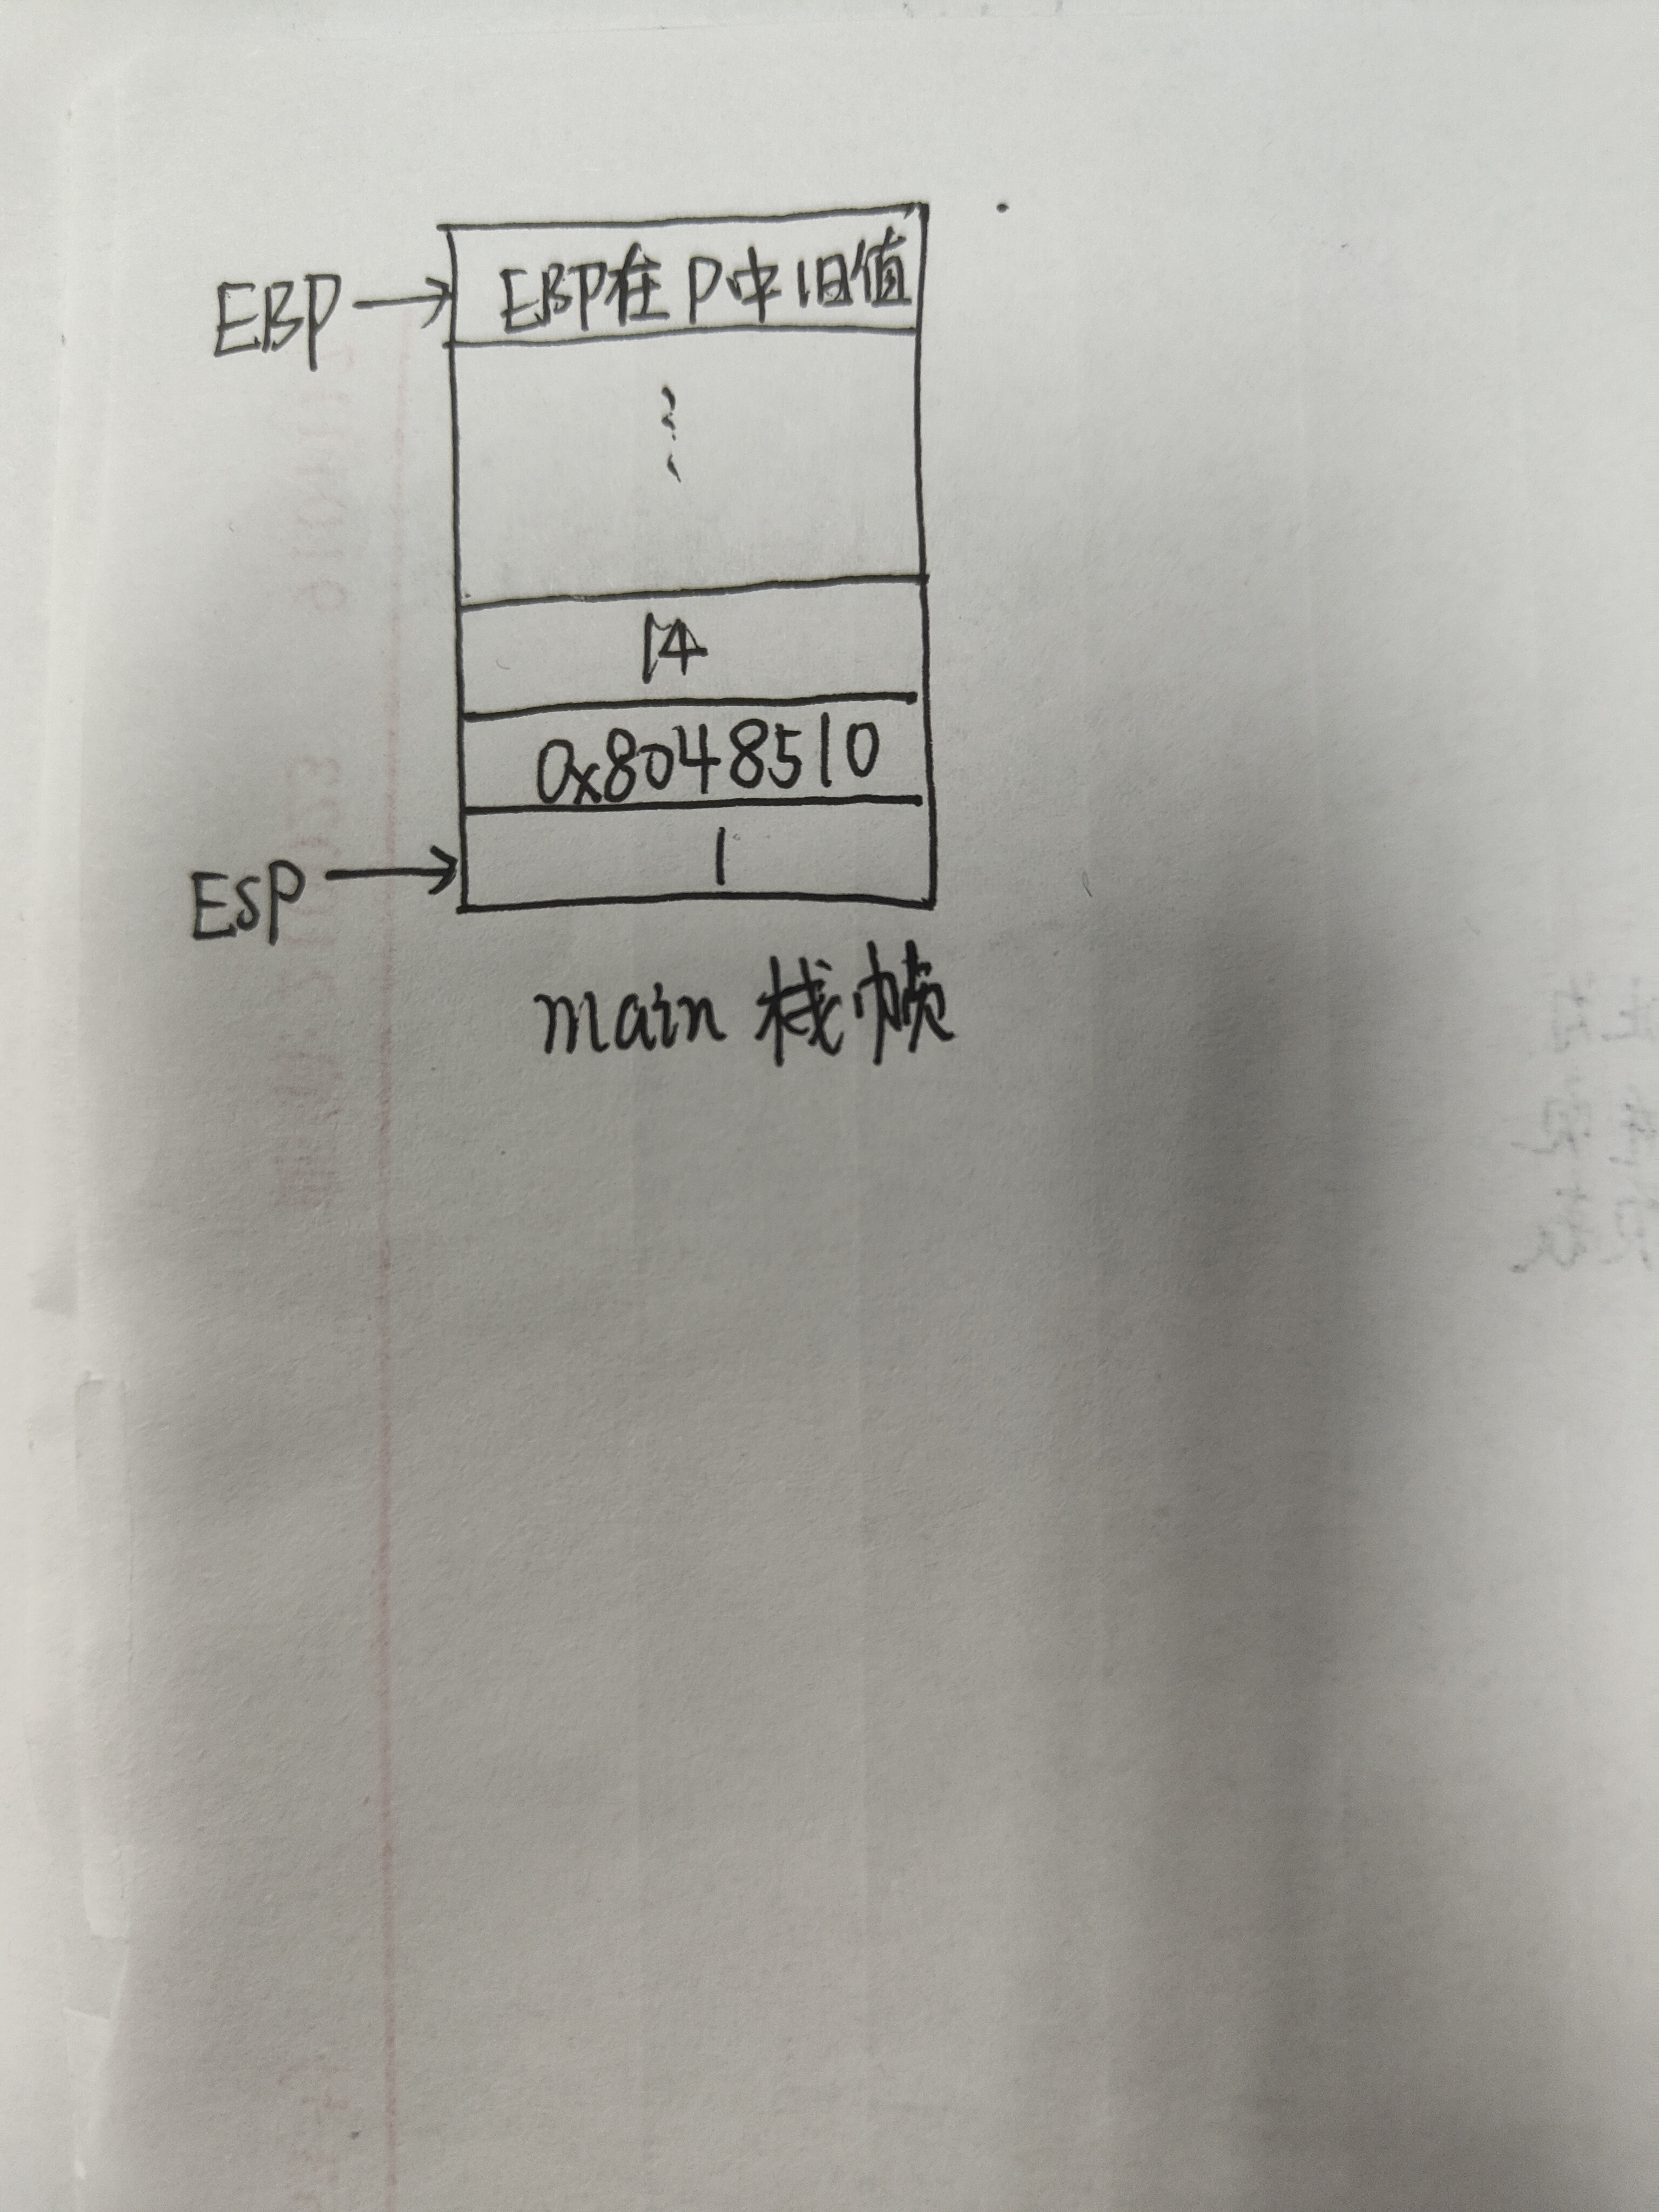
\includegraphics[width=4cm,height=4cm]{2.jpg}
\end{figure}

\subsection*{(2)}
\begin{figure}[h]
	\centering
	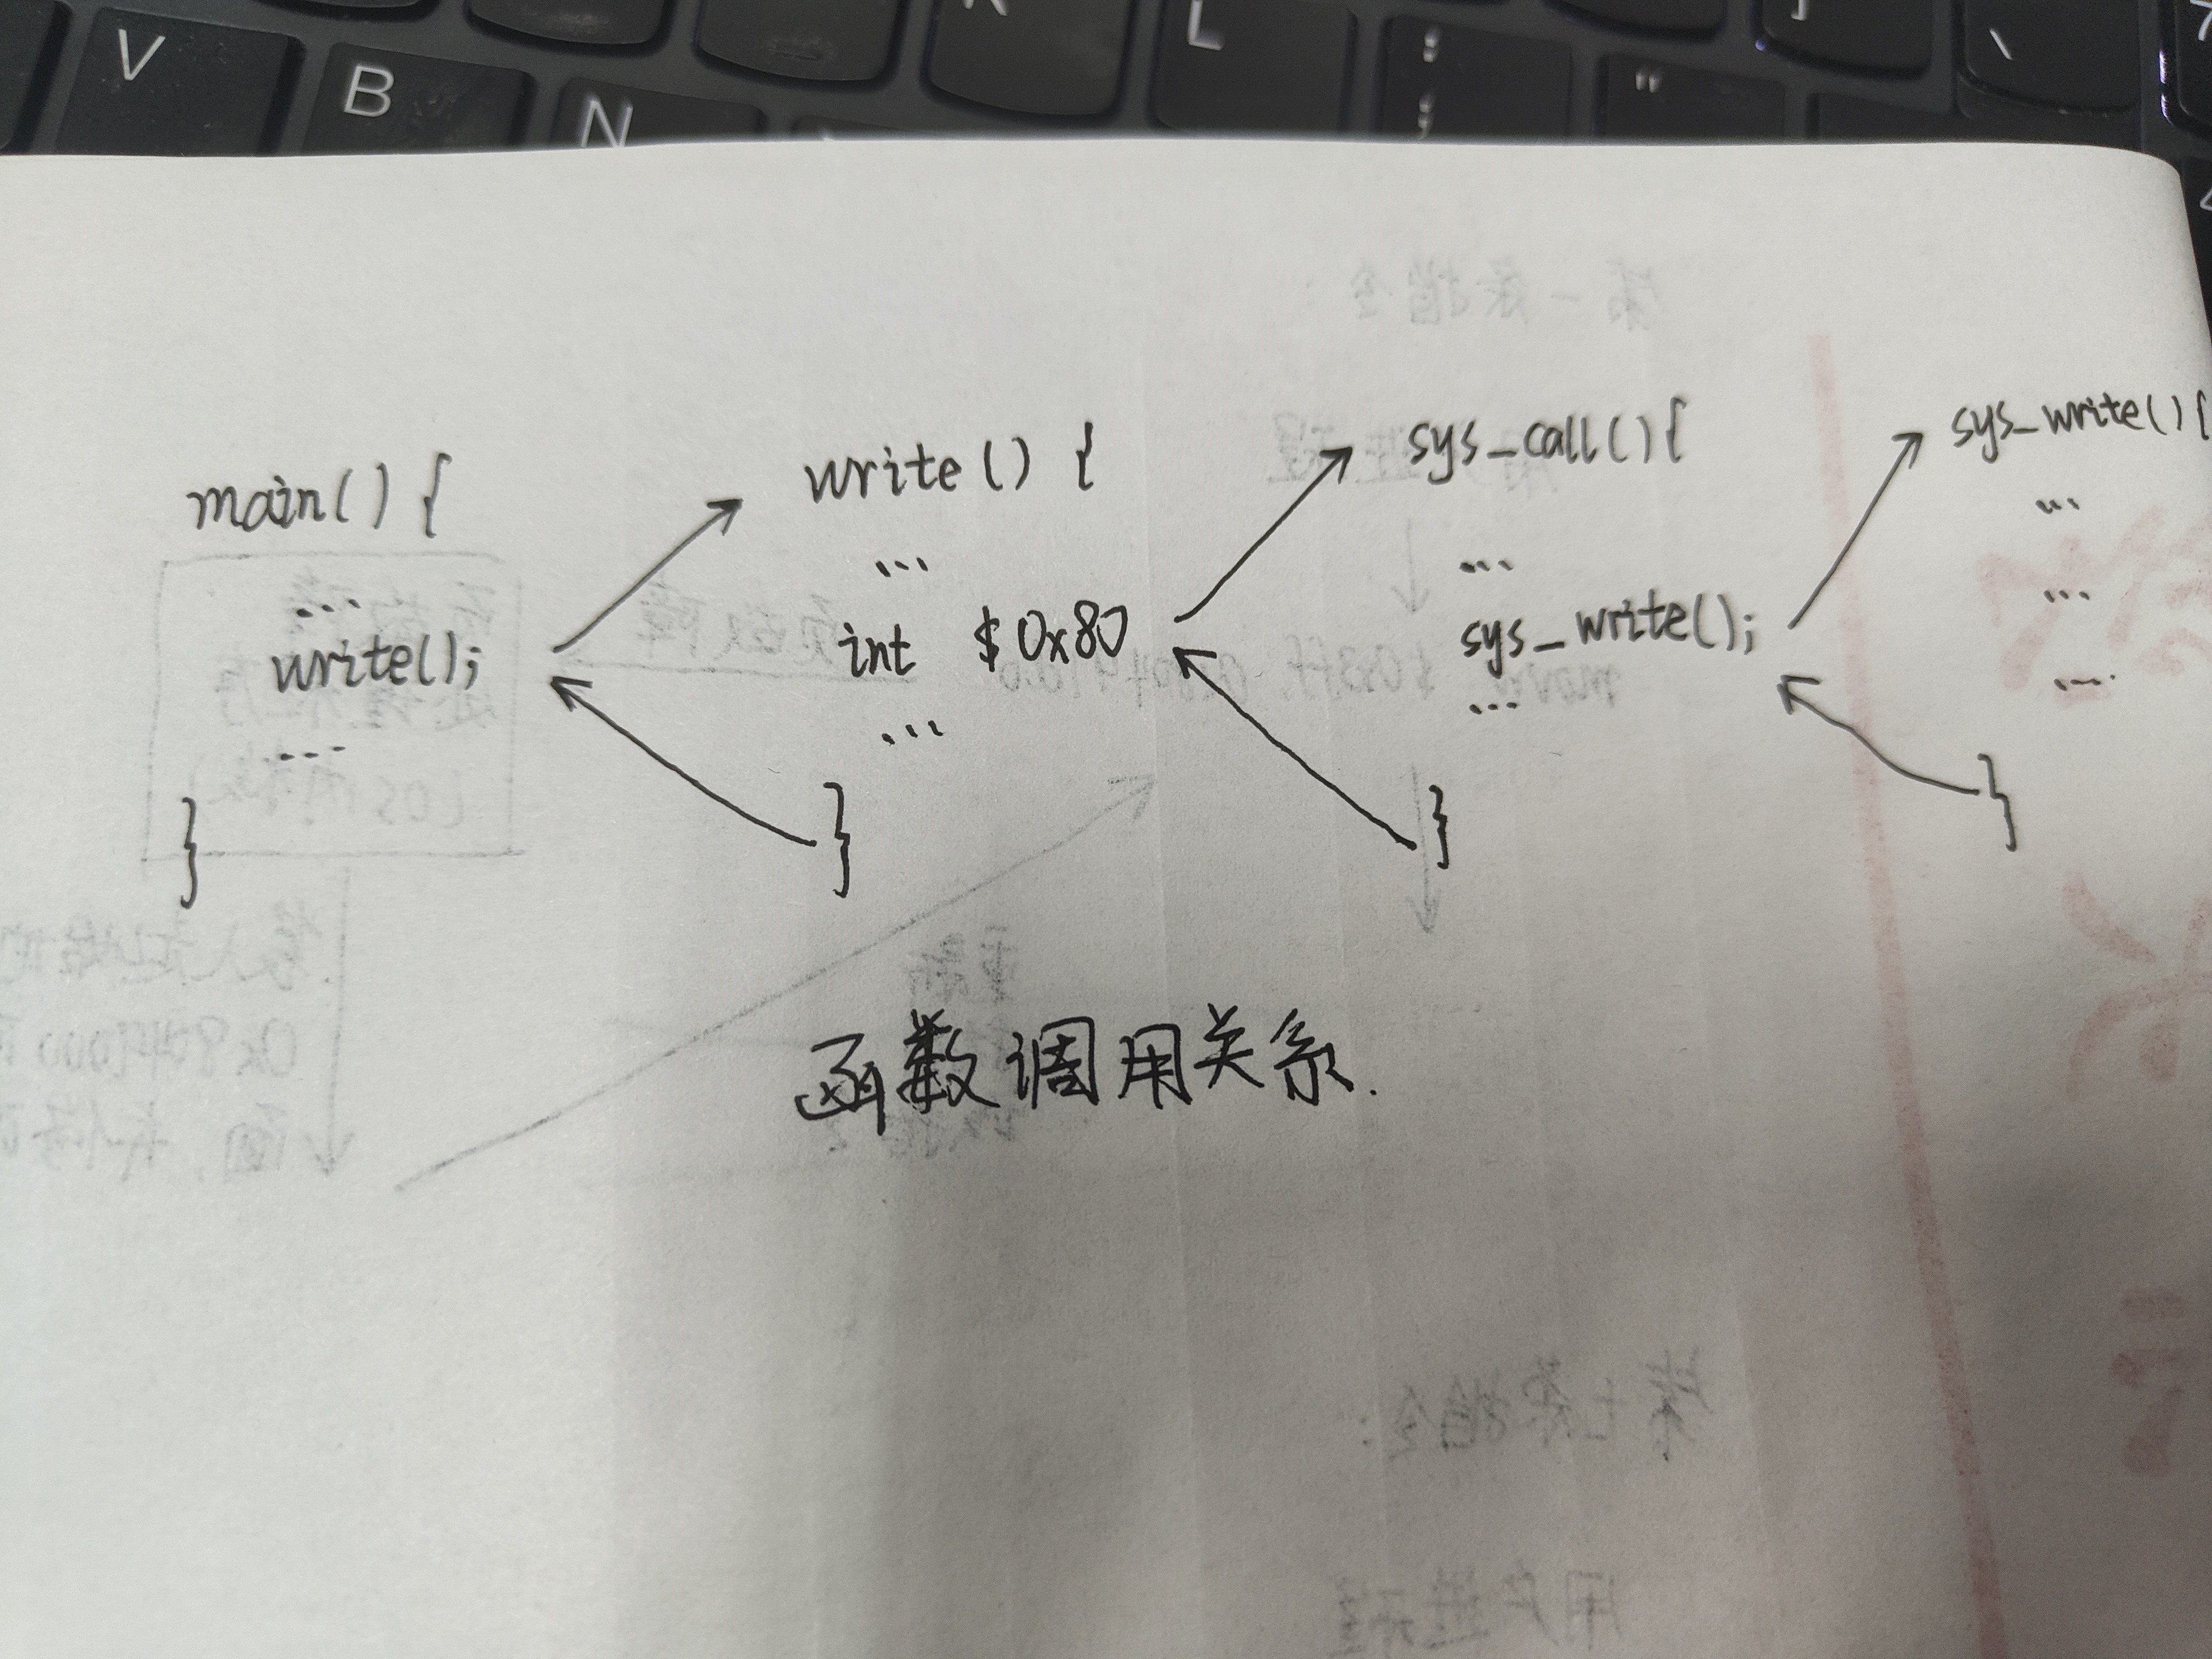
\includegraphics[width=8cm,height=4cm]{3.jpg}
\end{figure}
\newpage
\subsection*{(3)}
第3题采用汇编程序设计方式,只要参数不同,或者操作系统不同,就要重新编写不同的指令,
便捷性和可移植性差,但是省去了高级语言程序中的大量函数调用,所以执行时间最短。

本题直接调用write函数,当参数不同时,只要修改write()函数中的实参就可以,可移植性和便捷性比第3题的方式好。
\section*{P5}
\subsection*{(1)}
因为在hello.c中使用了标准库函数printf(),所以需要在hello.c的开头加"\#include <stdio.h>".

在stdio.h中有printf()函数的声明,在编译器预处理时,可以得到printf()函数的声明,从而获得printf符号的相关
信息,从而在链接时,能够从c库中得到printf()函数的定义。
\subsection*{(2)}
需要经过预处理、编译、汇编、链接才能生成可执行文件hello,然后才能启动hello程序。
预处理阶段主要是对带\#的语句进行处理;编译阶段主要是将预处理后的源代码编译成汇编语言程序;
汇编主要是将汇编语言程序转化为可重定位的机器语言程序;链接将多个可重定位目标文件以及库函数链接起来,
生成最终的可执行文件。
\subsection*{(3)}
因为print()函数默认的输出设备是标准输出设备stdout。
\subsection*{(4)}
机器码:48 65 6C 6C 6F 2C 77 6F 72 6C 64 0A 00(十六进制)。

这个0/1序列存放在hello.o的.rodata节中,是只读数据,这个0/1序列存放在可执行文件hello的只读代码段中。
\subsection*{(5)}
若采用静态链接,printf.o模块在静态库libc.a中,连接后,printf.o中的代码部分在虚拟地址空间的只读代码段中。
若采用动态链接,则函数printf()的代码在虚拟地址空间中的共享库映射区。
\subsection*{(6)}
// ebx入栈

// 将字符串长度14送edx

// 将字符串首地址送ecx

// 将文件描述符fd=1送ebx

// 将调用号4送eax

// 系统调用入口

// 恢复ebx的旧值

// 系统调用返回值与0xfffff001比较

// 大于等于是转出错处理

// 返回到调用write的过程

从倒数第3行汇编代码可以看出,系统调用返回的最大错误号是4095,故错误号范围是1-4095.
\subsection*{(7)}
第3题采用汇编程序设计方式,只要参数不同,或者操作系统不同,就要重新编写不同的指令,
便捷性和可移植性差,但是省去了高级语言程序中的大量函数调用,所以执行时间最短。

第4题直接调用write函数,只能在支持write系统调用的系统中执行,可移植性和便捷性不好。

本题采用的是C库函数调用,可以在不同的系统中执行,只有该系统配置了相关环境,所以便捷性和可移植性最好,
但是由于大量的函数调用,此方式编写的程序执行时间比前两种长。
\section*{P6}
\subsection*{(1)}
在内核的设备驱动程序。
\subsection*{(2)}
在内核的设备无关软件层。
\subsection*{(3)}
在用户I/O软件层。
\subsection*{(4)}
在内核的设备驱动程序层和中断服务程序层。
\subsection*{(5)}
在内核的设备驱动程序层和中断服务程序层。
\end{document}